
    To carry out data mining I used open source data mining software called Rapid Miner. I have also tried Weka, but I encountered problems while using it. 
    
    The Rapid Miner allows not only include the Weka classifiers into data mining process, but also has predefined interface for preprocessing text documents.
To top it all off, it can take advantage of multi-core processors and run computations in parallel.

Rapid Miner provides a workflow model where each process can be dragged and dropped on a canvas and then connected using arrows. It helps visualize the entire data mining task and provides a quick overview of the task at a glance. It's also worth mentioning that the interface works flawlessly, general help as well as contextual help is available at every step and it even has break points like most programming IDEs which allows to inspect intermediate results during a data mining process. It has excellent data import tools as well as reporting and visualization tools.

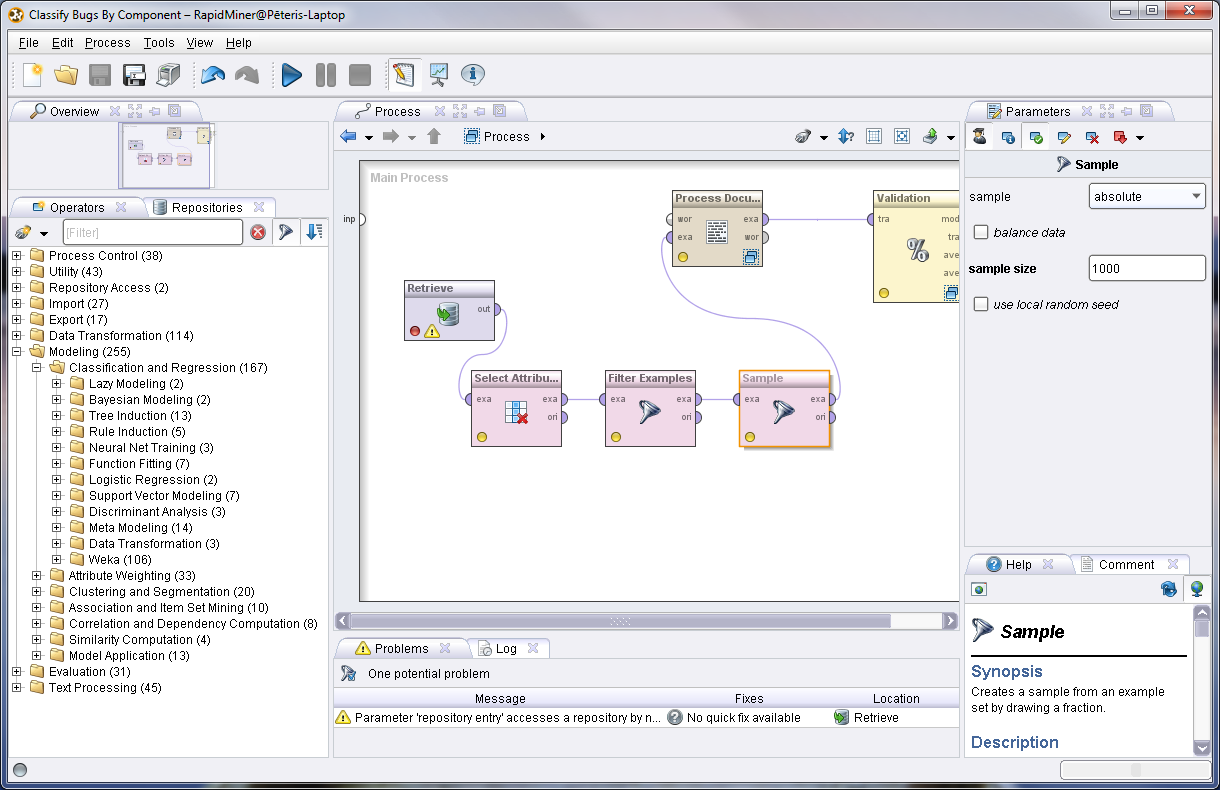
\includegraphics[scale=0.3]{ml3_tools_rapidminer}
